
\documentclass[UTF8,12pt,songti]{ctexart}

\title{}  %文章标题
\author{}   %作者的名称
\date{}       %日期
\usepackage[a4paper,left=25mm,right=25mm,top=25mm,bottom=25mm]{geometry}     %设置页面和边距
\usepackage{colortbl}
\usepackage{graphicx}
\usepackage{amsmath}
\usepackage{fancyhdr}
\usepackage{subfigure}
\usepackage{float}
\usepackage{listings}
\usepackage{xcolor}
\usepackage{pythonhighlight}
\pagestyle{fancy}
\lhead{}
\chead{}
\lhead{\#5182}
\rhead{\ }
\renewcommand{\headrulewidth}{0.4pt}

\setcounter{secnumdepth}{4}
\setcounter{tocdepth}{4}

\begin{document}

%生成目录设置
\maketitle        %显示标题
\renewcommand{\contentsname}{目录} %将content转为目录
\tableofcontents
\newpage

\section{问题重述}
\subsection{问题背景}
车险,即机动车辆保险。作为保险险种的一种,车险可以分散车辆在行驶过程中可能发生的未知风险和损失,减少投保人的财产损失。\par
近年来,随着我国保险业的稳步发展,机动车保险在我国的财险保费中所占的比例不断增加,投保率也呈上升趋势。我国目前的车险费率制度,大多符合“从车主义”,即保费的多少主要取决于车辆本身的情况。然而这样的定价机制是十分单调的,也不是十分合理。\par
未来车险业的发展趋势主要有以下两点:车险价格与驾驶行为密切相关、同价位车型车险价格完全不同。这一发展趋势表明,车主的个人信息将对车险价格产生更大的影响,车险价格不再单纯由车辆信息所决定。因此,针对不同客户定制独特的保险产品是十分必要的。而信息时代的到来,为这一需求提供了契机。车险企业可以利用数字化技术对用户数据进行分析,以更加精准地构建用户画像,制定营销和服务方案。
\subsection{问题描述}
基于问题背景和相关领域知识,本文试建立数学模型讨论下列问题:\par
1.根据附件中给出的客户个人信息,建立数学模型,对客户进行精准画像,进而预测客户的续保概率。\par
2.根据问题1中分析得到的客户续保概率预测模型,分析客户不同特征对客户续保概率的影响。提取其中的主要影响因子,并基于此为用户设计优惠和福利方案。
\section{模型假设}
1.假设所给数据中,除汽车品牌,汽车车系和新车价格以外的其他因素对于客户续保概率的影响相互独立。\par
2.假设在一年中不同的月份,客户的个人财务状况或其他情况不会对客户是否续保产生影响。
\section{符号说明}
\begin{table}[H]
\centering
\begin{tabular}{p{6cm} p{6cm} }% 通过添加 | 来表示是否需要绘制竖线
\hline  % 在表格最上方绘制横线
符号&含义\\
\hline
$x^{*}$&min-max标准化后得到的数据\\
\hline
min&样本数据最小值\\
\hline
max&样本数据最大值\\
\hline
P&概率\\
\hline
P(A\big|B)&条件概率\\
\hline
P(AB)&A,B事件同时发生的概率\\
\hline
A&在多层感知器中A表示某一神经元的输出\\
\hline
X&在多层感知器中X表示上一个神经元的输出\\
\hline % 在表格最下方绘制横线
\end{tabular}
\caption{符号说明}
\end{table}
\section{模型的建立与求解}
\subsection{问题1的分析与建模}
\subsubsection{问题1的分析}
结合问题1所要解决的问题,团队成员分析认为问题1是一个二分类问题。对于每个投保的用户而言,最终只存在续保和不续保这两种可能性,而用户是否续保又是由多个属性共同决定的。因此,这是一个典型的二分类问题。\par
经过分析,团队决定采用朴素贝叶斯分类模型、Logistic回归分类和多层感知器分类模型对训练数据集进行训练,并利用验证数据集进行模型验证。\par
题目所提供的用户信息,既包括数值信息,也包括文字信息。由于数值信息便于处理以及文字信息不满足Logistic回归分类和多层感知器分类模型对数据连续性的要求,需要对数据进行数值化处理。抽取数值化处理后得到的数据集的一部分组成训练集,对三种模型进行训练。最后利用验证集对三种训练模型进行验证。

\subsubsection{数据的预处理}
数据的预处理过程主要分为4个部分:数据的特征提取和清洗,数据中空值的填充,Logistic回归模型和多层感知器分类模型的数据预处理和朴素贝叶斯分类器的数据预处理。
\paragraph{数据的特征提取和清洗}  \quad \par     %空格加换行
为了对数据进行特征提取,我们首先对数据进行定性分析。\par
(1)由于“购买汽车保险”是一种计划消费行为,其消费往往不会受到“购买时间”所影响。“投保时间”不属于影响客户续保概率的主要因素。\par
(2)投保的车系,品牌和汽车价格,属于关联性极强的因素。在数据特征提取过程中,我们选取了其中特征性最强的汽车价格作为影响客户续保的主要因素。\par
(3)“被保人性别”是“客户类别”的更详细表示(其中“被保人性别”中的缺失值代表“客户类别”为机构),因此,只保留“被保人性别”作为影响客户续保概率的因素。\par
我们利用控制变量法,分别提取了每一个变量在每一种取值下,客户续保的概率。我们发现,所有车辆用途为“重、中型载货汽车”和“其他汽车”或车辆种类为“特种二挂车的客户均选择了续保。因此,我们认为,此类客户在未来续保的概率同样为100\%,然后继续对其余客户的数据进行处理。
\paragraph{数据中缺失值的填充} \quad \par
由于数据中存在大量缺失值,且缺失值同样代表了样本的重要特征。如“被保人性别”中的缺失值实际上代表了被保人“类型”为机构,因此不能直接清洗掉含有缺失值的数据,需要对缺失值进行填充。\par
(1)我们将“被保险人性别”中缺失值填充为“N”,代表机构类型。\par
(2)将“已决赔款”和“三者险保额”中缺失值填充为“0”,代表无已决赔款或三者险。\par
(3)将“风险类别”中缺失值填充为“0”,代表为进行风险评估。
\paragraph{Logistic回归模型和多层感知器分类模型的数据预处理}\quad \par
为了用Logistic回归模型和多层感知器分析模型进预测,必须将原始数据中的中文数据改为数值型数据。对于“是否续保”这样的0-1型数据,我们将其值映射为0和1。而对于具有多个不同离散值的属性,我们利用“one-hot”编码将其映射为多组0-1型数据。举例而言,对于”投保人”性别这一属性,我们将其映射为“投保人性别是否为男”“投保人性别是否为女”“投保人性别是否为NaN(机构)”三个0-1型属性。得到Logistic回归模型所需数据。
\begin{figure}[H]
\centering
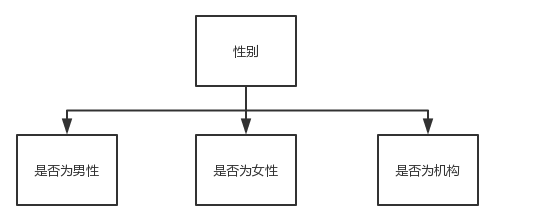
\includegraphics[width=14cm,height=6cm]{4-1-2-1.png}
\caption{one-hot处理投保人属性示意图}
\end{figure}
\par 在此基础上,对所有连续型数据,包括车龄,被保人年龄等,利用Min-Max标准化方法进行归一化处理,将连续型数据映射到0-1范围内,得到多层感知器分类模型所需数据。\par
\begin{equation}\label{min-max}
 x^{*}=\frac{x-min}{max-min}
\end{equation}
\quad \par 最终我们可以得到一个含有173项特征的特征向量用于训练Logistic回归模型和多层感知器分类模型。向量各项数据含义见附录一。
\paragraph{朴素贝叶斯分类器的数据预处理} \qquad  \par
为了使用朴素贝叶斯分类器对客户的投保概率进行预测,需要将连续型数据处理为离散型数据。根据连续特征值满足正态分布的特性,将连续型数据按区间进行划分。例如,新车购置价按照价格分为$<$5W,5W-7W,7W-10W,10W-15W,15W-20W,20W-30W,$>$30W共7个区间。
\subsubsection{Logistic回归分类的建立与求解}
\paragraph{模型原理} \quad \par
回归即通过大量数据已知数据对公式中的未知参数求解,形如$y=ax+b$中的a,b就是未知参数。而本题中的未知参数即各个客户投保属性前的参数,代表各属性对预测结果的影响比重。得到完整的公式后就可以进行预测,预测一般针对数值型数据,因此涉及数据的数值化处理。\par
Logistic回归的回归公式为$Z=w_{1}x_{1}+w_{2}x_{2}+w_{3}x_{3}+$…$+w_{a}x_{a}+b$,通过训练将函数值Z映射到不同的分类区间,针对本题即为两个区间,代表投保和不投保。将函数值映射到不同分类区间需要利用sigmoid函数。
\begin{equation}\label{logistic1}
f(x)=\frac{1}{1+e^{-x}}
\end{equation}
\par 该函数可将数据映射到[0,1]上。设置一个阈值,根据阈值将数据划分为两类。之后根据结果不断拟合,寻找最佳拟合。\par
分类函数构造完成后,需要引入损失函数,该函数表示预测的输出(h)与训练数据类别(y)之间的偏差。综合考虑所有训练数据的损失,得到误差函数J(x)。J(x)函数值越小代表预测函数越准确。找到J(x)的最小值即获得了最准确的预测函数。\par
整个Logistic回归分类模型的分析过程见下图。
\begin{figure}[H]
\centering
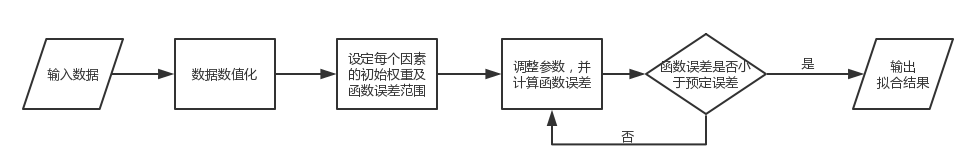
\includegraphics[width=18cm,height=3.5cm]{4-1-3-1.png}
\caption{Logistic回归分类模型流程图}
\end{figure}
\paragraph{模型建立与求解} \quad \\
(1)确定预测函数\par
预测函数原型为sigmoid函数。根据拟合结果,预测函数大致为线性函数。\\
(2)构造损失函数和Logistic回归分类模型\par
损失函数选取Python3中Sklearn库中Logistic Regression函数,利用损失函数构造Logistic回归分类模型,模型共包含173项参数。其中重要参数表如下。
\begin{table}[H]
\centering
\begin{tabular}{|p{4cm} |p{10cm}|  }% 通过添加 | 来表示是否需要绘制竖线
\hline  % 在表格最上方绘制横线
参数名称&含义及设定值 \\
\hline
tol&迭代终止判断的误差范围,设置为$(0.1)^{7}$ \\
\hline
max\_iter&最大迭代次数,设置为100000 \\
\hline
penalty&正则化类型,设置为l2\\
\hline
dual&用于liblinear解决器中L2正则化,设置为false\\
\hline
class\_weight&每种属性的权重,初始设置为1,根据训练结果调整\\
\hline % 在表格最下方绘制横线
\end{tabular}
\caption{Logistic模型重要参数}
\end{table}
(3)梯度下降法减小误差\par
利用LR自带的Gradient Descent算法对损失函数的均值J(x)进行处理,找到J(x)的最小值,修正模型。\\
(4)模型求解结果\par
将总数据集均分为10组,选取其中的9组对模型进行训练。最终得到准确率为99.526934\%的Logistic回归分类模型。
\subsubsection{朴素贝叶斯分类模型的建立与求解}
\paragraph{模型原理} \quad \\
(1)算法简介\par
贝叶斯算法是以贝叶斯定理为基础的,通过概率求解,预测发生概率,以此将最终结果进行分类(更可能发生|更可能不发生)的算法。而朴素贝叶斯,是该分类算法中比较基础的一种。\par
贝叶斯定理基本求解公式为:
\begin{equation}\label{bayes1}
P(A\big|B)=\frac{P(AB)}{P(B)}=\frac{P(B\big|A)*P(A)}{P(B)}
\end{equation}
\par 其中,待分类集A即为我们要预测的结果,特征属性集B就是我们已知的、或通过某些方式可知的其他因素,B中每个特征属性集的叠加将导致我们对A的选择发生改变。通过上述公式,计算并选择待分类集A中条件概率最大的类别,作为预测结果。\\
(2)算法定义 \par
1.设$X=\left \{ x_{1},x_{2},...,x_{m} \right \}$为一个待分类集,而每个a 都是X的一个特征属性\par
2.设类别集合$C=\left \{ y_{1},y_{2},...,y_{n} \right \}$ \par
3.计算$P(y_{1}\big|X),P(y_{2}\big|X),P(y_{3}\big|X)$...$P(y_{n}\big|X)$ \par
4.若$P(y_{k}\big|X)=\max\left \{ P(y_{1}\big|X),P(y_{2}\big|X),P(y_{3}\big|X)...P(y_{n}\big|X) \right \} $,则$ X \epsilon y_{k}$  \\
(3)计算方法  \par
1.找到一个已知结果的待分类项集合,作为训练样本。\par
2.统计得到在各类别下各特种属性的条件概率估计:\[P(a_{1}\big|y_{1}),P(a_{2}\big|y_{1}),...,P(a_{m}\big|y_{1}),P(a_{1}\big|y_{2}),P(a_{2}\big|y_{2}),...,P(a_{m}\big|y_{n})\] \par
3.若各项特征值间相互独立,即
\begin{equation}\label{bayes2}
  P(\prod_{i=1}^{m}a_{i})=\prod_{i=1}^{m}P(a_{i})
\end{equation}
\par则有
\begin{equation}\label{bayes3}
  P(y_{i}\big|x)=\frac{P(x\big|y_{i})P(y_{i})}{P(x)}
\end{equation}
\par
4.又因为分母对于所有的类别都为同一个常数,那么我们只需求出分子最大值即可,因此有:
\begin{equation}\label{bayes4}
 P(x_{i}\big|y_{i})P(y_{i})=P(a_{1}\big|y_{i})P(a_{2}\big|y_{i})P(a_{3}\big|y_{i})...P(a_{m}\big|y_{i})=P(y_{i})\prod_{j=1}^{m}P(a_{j}\big|y_{i})
\end{equation}
(4)特征属性划分及Laplace校准\par
1.若特征值连续,通常假定其值服从正态分布,即
\begin{equation}\label{bayes5}
  g(x,\eta ,\sigma )=\frac{1}{\sqrt{2\pi }\sigma }e^{\frac{-(x-\eta )^{2}}{2\sigma ^{2}}}
\end{equation}
\par 而
\begin{equation}\label{bayes6}
  P(a_{k}\big|y_{i})=g(a_{k},\eta _{y_{i}},\sigma _{y_{i}})
\end{equation}
\par
由此我们将 “新车购置价”,“被保险人年龄”,“签单保费”以及“已决赔款”四个属性特征值重新定义、划分区间,使之能够更加准确的描述他们对于“是否续保”这一待分类集的变化趋势。\par
2.在有些实例中,某些因素的概率为0 ,即$P(a_i\left|y_j\right)=0$。这时,我们引入Laplace校准\footnote{当训练样本集充分大时,Laplace校准并不会对结果产生影响。},对每类别下所有划分的计数加一。
\paragraph{模型建立与求解} \quad \\
(1)模型预处理\par
在本题中, 使用朴素贝叶斯公式,基本模型如下:\par
待分类集{“是否续保”}\par
属性特征值\footnote{“保单号”作为数据库主键约束,与待分类集无关,舍去;“终止日期”为“起保日期”后一年,该因素对待分类集的影响与“起保日期”一致,舍去}{“起保日期”\footnote{经研究,“是否续保” 对“起保日期”不敏感,故以年份重新划分起保日期,详见附录} ,“渠道”,“品牌”,“车系”,“保单性质”,“续保年”,“投保类别”,“是否本省车牌”,“使用性质”,“车辆种类”,“车辆用途”,“新车购置价”,“被保险人年龄”,“签单保费”,“已决赔款”\footnote{因为“新车购置价”,“被保险人年龄”,“签单保费”以及“已决赔款”四个属性特征值连续,故按照高斯分布将其重新划分类别。除这四种外,按照数据源的类别计算。},“车龄”,“险种”,“NCD”,“风险类别”,“客户类别”,“被保险人性别”,“是否投保车损”,“是否投保车上人员”,“是否投保盗抢”,“三者险保额”,“立案件数”} 共计26项\footnote{各属性特征值类别数见附录}\\
(2)计算概率 \par
我们使用Oracle数据库读入数据源,经过筛选得出每个属性的每个类别的结果\footnote{各类别概率由于数据量过大不再列出,核心查询SQL语句见附录}。
\subsubsection{多层感知器分类模型的建立与求解}
\paragraph{模型原理}  \quad \par
多层感知器(Multi-Layer Perceptron,MLP)也叫人工神经网络(Artificial Neural Network,ANN),除了输入输出层,它中间可以有多个隐含层。在输入层和隐含层之间的神经元中,存在数据传递。数据传递关系如公式所示: 对于任一层
\begin{equation}\label{MLP1}
Z = W_1 * X + b
\end{equation}
\begin{equation}\label{MLP2}
A = sigmoid(Z)
\end{equation}
\par 然后不断利用代价函数修正每个神经元中的系数w和b。最终得到可以正确对样本进行分类的神经网络
\begin{figure}[H]
\centering
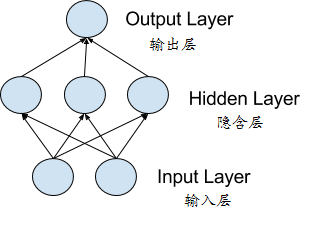
\includegraphics[width=10cm,height=7cm]{4-1-5-1.png}
\caption{多层感知器分类模型示意图}
\end{figure}
\paragraph{模型建立与求解}  \quad \par
我们利用python3 sklearn库中的MLPClassifier函数,建立一个具有1个隐藏层200个神经元的多层感知器。损失函数选择协方差,其他参数及设定值见下表。
\begin{table}[H]
\centering
\begin{tabular}{|p{6cm} |p{6cm} | }% 通过添加 | 来表示是否需要绘制竖线
\hline  % 在表格最上方绘制横线
参数名称&设定值 \\
\hline
初始学习率&0.01 \\
\hline
激活函数&relu \\
\hline
最大迭代次数&2000\\
\hline % 在表格最下方绘制横线
\end{tabular}
\caption{多层感知器模型参数设置}
\end{table}
\par然后将数据中的前50000组数据作为训练数据输入模型。最终得到准确率为99.665\%的神经网络模型。      将任一客户数据输入模型后,可以得到客户续保概率为99.665\%或不续保概率为99.665\%,完成对用户画像的精准绘制。
\subsection{问题2的分析与建模}
\subsubsection{问题2的分析}
问题2是在问题1的基础上,要求提取出续保概率较大的客户所具有的的特征,并求出其中对客户续保概率影响最大的几个特征。我们可以首先利用问题1求解过程中数据预处理部分得到的在控制变量情况下的续保概率情况,结合朴素贝叶斯分类模型,得到最优质客户的用户画像。再利用问题1求解过程中Logistic回归模型中的不同参数的系数和不同参数的数值大小情况,确定各个特征中影响最明显的几个变量,最后确定有效的营销方案。
\subsubsection{模型建立与求解}
我们首先利用问题1求解过程中数据预处理部分得到的在控制变量情况下的续保概率分布,结合朴素贝叶斯分类模型,得到最优质客户的用户画像。\par
\begin{figure}[H]
\centering
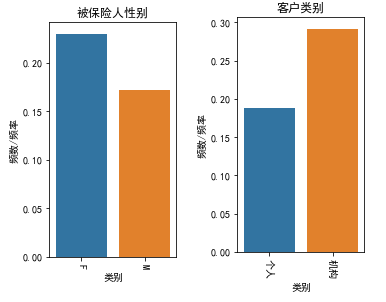
\includegraphics[width=8cm,height=6cm]{4-2-2-1.png}
\caption{被保险人性别和客户类别概率分布图}
\end{figure}
\begin{figure}[H]
\centering
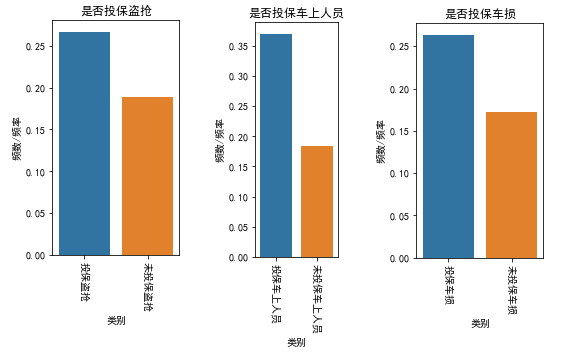
\includegraphics[width=12cm,height=9cm]{4-2-2-2.png}
\caption{是否投保盗抢,车上人员,车损概率分布图}
\end{figure}
\begin{figure}[H]
\centering
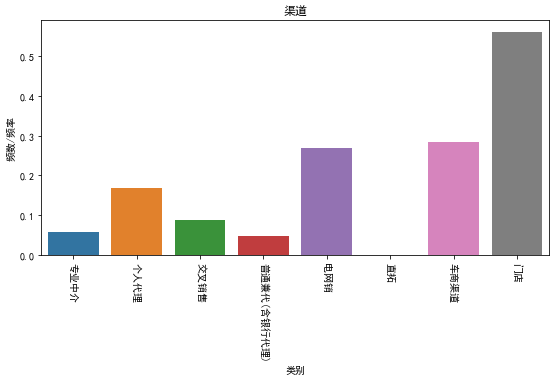
\includegraphics[width=12cm,height=9cm]{4-2-2-3.png}
\caption{渠道概率分布图}
\end{figure}
\begin{figure}[H]
\centering
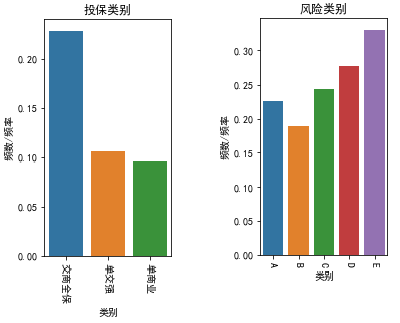
\includegraphics[width=12cm,height=9cm]{4-2-2-4.png}
\caption{投保类别和风险类别概率分布图}
\end{figure}
\begin{figure}[H]
\centering
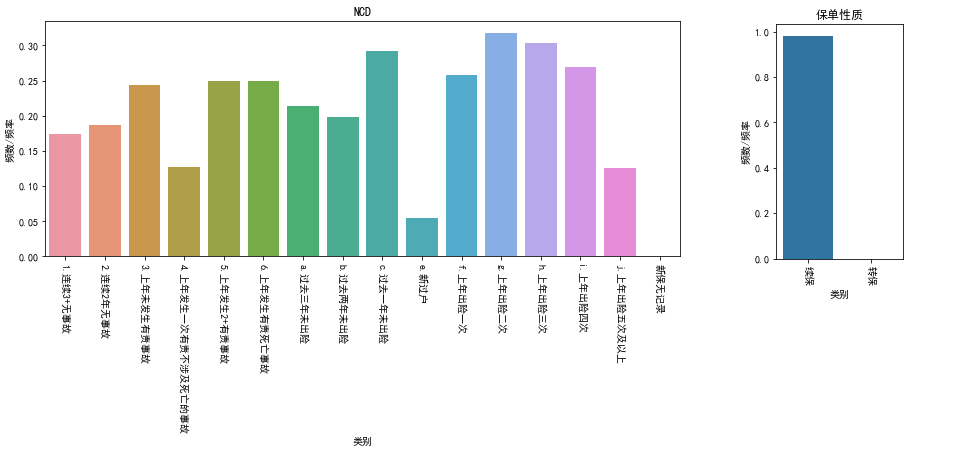
\includegraphics[width=18cm,height=10cm]{4-2-2-5.png}
\caption{NCD和保单性质概率分布图}
\end{figure}
\par 最终得到的最优质客户具有以下特征:\par
\begin{table}[H]
\centering
\begin{tabular}{|p{6cm} |p{6cm} | }% 通过添加 | 来表示是否需要绘制竖线
\hline  % 在表格最上方绘制横线
特征&特征值 \\
\hline
新车购置价&10W-15W \\
\hline
已决赔款&空 \\
\hline
签单保费&800-900\\
\hline
三者险保额&空\\
\hline
被保险人年龄&30-35\\
\hline
车辆种类&10吨及10吨以上挂车\\
\hline
渠道&非门店\\
\hline % 在表格最下方绘制横线
\end{tabular}
\caption{最优质客户特征表}
\end{table}
\par
然后利用Logistic回归模型中的不同参数的系数和不同参数的均值相乘的结果排序,确定各个特征中影响最明显的几个变量。尽管这样得到的排序可能与真实因素的影响存在偏差,但是由于我们提取的是多个变量,而非单个最重要的影响因素,这样的误差不会影响到模型结果。最终,我们得到几个影响客户是否续保的最关键因素:[“是否10吨以上货车”,“上年事故情况”,“是否本省车牌”,“是否为轻微型载货汽车”,“是否为门店渠道”,“是否营业货车”]。其中,各因素对客户是否续保的影响如下:\par
(1)是否10吨以上货车:车型为10吨以上货车的客户,续保概率更大。\par
(2)上年事故情况:上年发生2+有责事故的客户,续保概率更大。\par
(3)是否本省车牌:车牌为本省的客户,续保概率更大 。\par
(4)是否为轻微型载货汽车:车型为轻微型载货汽车的客户,续保概率更大。\par
(5)是否为门店渠道:通过非门店渠道的客户,续保概率更大。\par
(6)是否营业货车:拥有营业货车的客户,续保概率更大。
\par
根据以上建模分析结果和市场调研,我们制定如下优惠政策:\par
(1)加强对于保单到期的客户的宣传,同时加强对于新客户的福利待遇,如折扣,减保额,发放优惠券等。\par
(2)设置信誉额度,对于去年未发生任何事故情况的车辆有额外优惠。同时对于去年发生2起以上有责交通事故的车辆,扣除一定的信誉额度,增加其保额。\par
(3)对于本省车牌或带拖挂汽车,轻微型载货汽车,营业货车等投保,增加优惠,如削减保额,延长保险年限等。\par
(4)对于轻微型载货汽车,营业货车,增加优惠。\par
(5)对于转保的客户,增加一定额度的手续费。
\section{模型验证}
\subsection{Logistic回归分类模型的验证}
我们使用交叉验证的方法对Logistic回归分类模型进行了验证。首先将数据集均匀划分为10组,每次使用9组数据进行训练,并使用1组数据进行检验,每次验证的准确率如表所示:
\begin{table}[H]
\centering
\begin{tabular}{|p{6cm} |p{6cm} | }% 通过添加 | 来表示是否需要绘制竖线
\hline  % 在表格最上方绘制横线
第1次验证&0.99526934 \\
\hline
第2次验证&0.99649016 \\
\hline
第3次验证&0.99633756 \\
\hline
第4次验证&0.99557455\\
\hline
第5次验证&0.99587975\\
\hline
第6次验证&0.99587912\\
\hline
第7次验证&0.99633700\\
\hline
第8次验证&0.99633700\\
\hline
第9次验证&0.99679438\\
\hline
第10次验证&0.99679438\\
\hline % 在表格最下方绘制横线
\end{tabular}
\caption{Logistic回归分类模型验证准确率}
\end{table}
\par 每一次验证都得到了较好的结果,证明模型有效。
\subsection{朴素贝叶斯模型的验证}
编写Python程序\footnote{Python源码见附录}进行验证。经测试,准确率为99.50408\%。
\subsection{多层感知器分类模型的验证}
我们利用“留出验证”的方法对多层感知机分类模型进行验证。我们将前50000组数据作为训练集输入模型进行训练,然后将剩下的数据作为测试集。测试集准确度为0.9966499162479062,属于较高水平,证明模型有效。
\subsection{模型验证综述}
三者间能够互相印证,尤其是Logistic回归模型进行了交叉验证,证明较高的准确率并非是过拟合造成的,而是因为数据本身具有较强的规律性。
\section{模型评价及改进}
\subsection{模型优点}
(1)数据预处理合理:我们对原始数据进行了有效的数值化处理。使得我们的模型均取得了较好的效果。\par
(2)无论模型对数据的要求是离散型还是连续型,或要求归一化处理,处理后的数据都可以直接用以训练。为未来的改进留下了空间。\par
(3)模型选用合理:我们经过研究分析,最终使用了朴素贝叶斯分类算法,logistic回归,以及多层感知器这三种模型来进行预测,结果准确率均大于99\%。
\subsection{模型缺点}
(1)多个模型之间联系较少,工作具有重复性。\par
(2)对于多层感知器分类模型,没有进行交叉验证,验证力度不足。
\subsection{模型改进}
(1)可以利用boost算法对三个模型的预测结果进行整合,获得更好的预测模型。\par
(2)多层感知器模型可以改进为隐藏层更多的神经网络模型,利用深度学习来获取更高的准确率。\par
(3)可以引入更多的分类模型和方法,如决策树和支持向量自动机。
\section{参考文献}
[1]Kose I,Gokturk M,Kilic K An interactive machine-learning-based electronic fraud and abuse detection system in healthcare insurance[J]. Applied Soft Computing, 2015, 36:S1568494615004585 \par
[2]周志华  机器学习[M] 清华大学出版社,2017-06-01\par
[3]司守奎,孙兆亮等著. 数学建模算法与应用(第二版)[M].国防工业出版社,2015-04-01 \par
[4]Frank R.Giordano,William P.Fox等著,叶其孝等 译. 数学建模(第五版)[M].机械工业出版社,2014-10-01\par
\section{附录}
\subsection{朴素贝叶斯模型部分代码实现} \quad \\
以被保险人年龄为19为例
\begin{python}
 elif i==19:
            tempValue=float(testValue)
            if tempValue>50:
                YRate=YRate*float(dFY[curSecondColumnY][7])
                NRate=NRate*float(dFN[curSecondColumnN][7])
            elif tempValue<25:
                YRate=YRate*float(dFY[curSecondColumnY][1])
                NRate=NRate*float(dFN[curSecondColumnN][1])
            elif tempValue>= 25 and tempValue<30:
                YRate=YRate*float(dFY[curSecondColumnY][2])
                NRate=NRate*float(dFN[curSecondColumnN][2])
            elif tempValue>= 30 and tempValue<35:
                YRate=YRate*float(dFY[curSecondColumnY][3])
                NRate=NRate*float(dFN[curSecondColumnN][3])
            elif tempValue>= 35 and tempValue<40:
                YRate=YRate*float(dFY[curSecondColumnY][4])
                NRate=NRate*float(dFN[curSecondColumnN][4])
            elif tempValue>= 40 and tempValue<45:
                YRate=YRate*float(dFY[curSecondColumnY][5])
                NRate=NRate*float(dFN[curSecondColumnN][5])
            elif tempValue>= 45 and tempValue<50:
                YRate=YRate*float(dFY[curSecondColumnY][6])
                NRate=NRate*float(dFN[curSecondColumnN][6])
            else :
                print("null")

\end{python}
\end{document}

